\documentclass[unicode]{beamer}
\usepackage[T2A]{fontenc}
\usepackage[utf8]{inputenc}
\usepackage[russian]{babel}
\usepackage{cmap}
\usepackage{amssymb,amsfonts,amsmath,mathtext}
\usepackage{graphicx}
% XeTeX packages
\usepackage{lmodern} % or install lmodern and remove cm-default opt
\usepackage{xunicode} % some extra unicode support
\usepackage{xltxtra} % \XeLaTeX macro
\defaultfontfeatures{Scale=MatchLowercase,Mapping=tex-text}
\usepackage{verbatim} 

\setromanfont{Charis SIL}
\setsansfont{Charis SIL}
\setmonofont{Charis SIL}

\usepackage{geometry}
\geometry{left=0mm}
\geometry{right=0mm}
\geometry{top=0cm}
\geometry{bottom=0cm}

\usepackage{array}

\setbeamerfont{institute}{size=\normalsize}
\graphicspath{{pictures/}}
\usetheme{CambridgeUS}
\useoutertheme{shadow}
\useinnertheme{rounded}
\usecolortheme{beaver}
\usefonttheme{professionalfonts}


\title[Разработка расширений для системы управления проектами Redmine]{
Разработка расширений для системы управления проектами Redmine
}
\author[Кандауров О.\,В.]{Студент 5-го курса О. Кандауров}
\institute{
Научный руководитель: ст. преподаватель Парамонов~И.\,В.
}
\date{}
\begin{document}
\maketitle

\begin{frame}
\transwipe[direction=90]
\frametitle{Системы управления проектами}
\begin{columns}
\begin{column}{0.45\textwidth}
\begin{block}{Функциональность}
\begin{itemize}
  \item Планирование
  \item Постановка задач
  \item Оценка и разработка
  \item Управление бюджетом
  \item Распределение ресурсов
  \item Взаимодействие
  \item Документирование
\end{itemize}
\end{block}
\end{column}
\begin{column}{0.55\textwidth}
\centerline{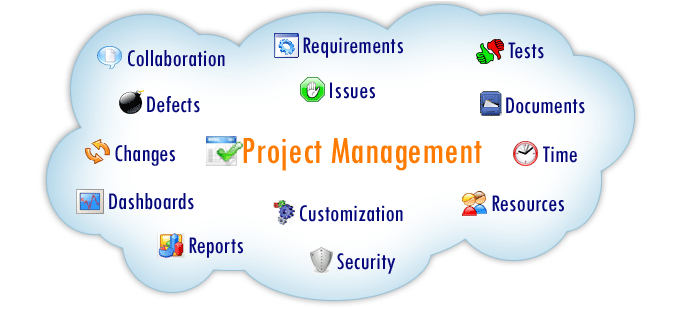
\includegraphics[width=1\textwidth]{project-management-software.png}}
\end{column}
\end{columns}
\end{frame}

\begin{comment}

Разработка и управление проектами является сложным процессом, облегчить
выполнение которого могут системы управления проектами. Системы управления
проектами - это программные системы, которые позволяют контролировать все
аспекты связанные с разработкой проектов. Основная задача систем управления
проектами, заключается в том, чтобы уменьшить сложность ведения крупных
проектов и способствовать эффективному управлению несколькими проектами.

\end{comment}


\begin{frame}
\transwipe[direction=90]
\frametitle{Redmine}
\centerline{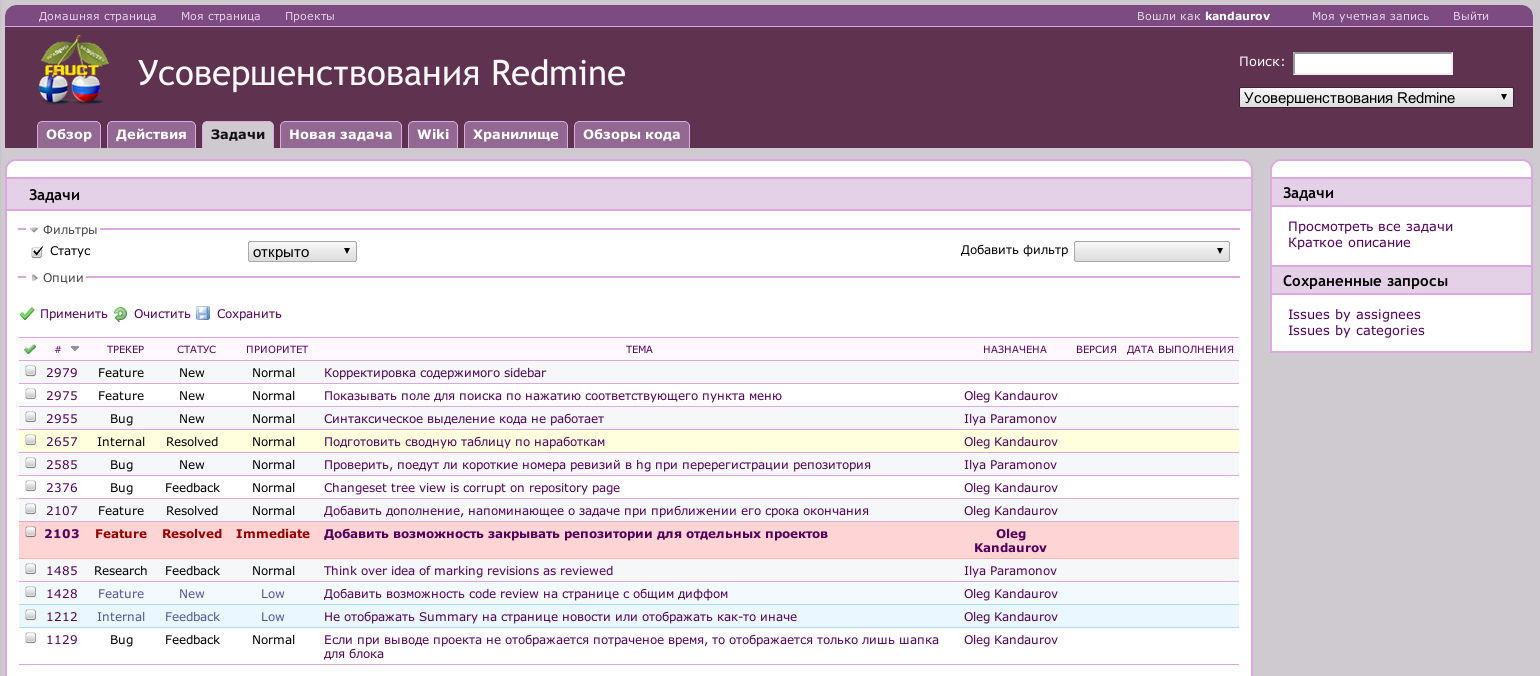
\includegraphics[scale=0.32]{redmine-issues.png}}
\end{frame}

\begin{comment}

Redmine это система управления проектами, которая позволяет управлять процессом
разработки на всех этапах жизненного цикла. На слайде показан проект в системе
Redmine в котором осуществлялась управление задачами в рамках диплома.
Redmine - это веб-приложение, основными достоинствами которого являются богатая
функциональность, расширяемость и доступные исходные коды. Данные качества
продукта позволяют производить его доработку в соответствии с нуждами
организации.

\end{comment}

\begin{frame}
\transwipe[direction=90]
\frametitle{Постановка задачи}
\begin{block}{}
\begin{itemize}
  \item Реализовать дополнительный функционал
  \begin{itemize}
    \item Ограничение доступа к вики-страницам
    \item Ограничение доступа к репозиториям
    \item Рассылка уведомлений о приближающихся задачах
    \item Изображения-ссылки в боковой панели
    \item Тип задачи при составлении обзора кода
    \item Механизм позиционирования всплывающего календаря
  \end{itemize}
  \item Создать инфраструктуру, упрощающую поддержку расширений;
  \item Разместить расширения в открытом доступе
\end{itemize}
\end{block}
\end{frame}

\begin{comment}

Ярославская лаборатория FRUCT ведёт исследования в области
мобильных систем и технологий, а также разрабатывает прототипы программных
продуктов, основанные на этих исследованиях. На текущий момент активны
более 10 проектов, участниками которых являются студенты и аспиранты факультета
ИВТ.

Система управления проектами Redmine обладает рядом ограничений, которые в
затрудняют процесс управления проектами, поскольку не отражают особенности
данного процесса в лаборатории. Поэтому в данной работе ставится задача по
разработке ряда расширений, повышающих эффективность работы с системой и
реализующих дополнительный функционал.

Помимо центральной задачи разработки расширений в работе также решаются две
дополнительные задачи:
\begin{itemize}
  \item создание инфраструктуры, упрощающей поддержку расширений;
  \item размещение расширений в открытом доступе.
\end{itemize}

Первая из этих задач возникает потому, что Redmine регулярно обновляется и
возможно, что одно из таких обновлений сделает неработоспособными часть
расширений и они потребуют исправлений. Исходя из этого, необходимо разработать
механизм позволяющий эффективно управлять итеративной разработкой и поддержкой
большого количества расширений.

Решение второй задачи желательно потому, что Redmine "--- это Open Source
проект, разививаемый разработчиками по всему миру. Открыв доступ к расширениям,
можно привлечь сторонних разработчиков, которые помогут их развивать. Для
достижения этого необходимо, чтобы разработанные расширения быть выложены в
открытый доступ.

\end{comment}

\begin{frame}
\transwipe[direction=90]
\frametitle{Разработка плагина}
\begin{block}{Плагин, ограничивающий доступ к вики-страницам}
\begin{itemize}
  \item Регистрация плагина
  \item Миграция базы данных
  \item Система контроля доступа
  \item Расширение классов во время выполнения
  \item Маршрутизация запросов
  \item Hooks
\end{itemize}
\end{block}
\end{frame}

\begin{comment}

Реализация будет рассказана на примере одного из расширений. Вики-страница это
страница на сайте, содержимое которой пользователи могут самостоятельно
изменять с помощью инструментов предоставляемых сайтом. Форматирование текста
на таких страницах производится использованием специального языка разметки.
Система контроля доступа в Redmine не даёт возможности ограничить просмотр лишь
отдельных вики-страниц в проекте. Из-за чего возникла потребность добавить
функционал, который бы контроллировал доступ к отдельным страницам. Данная
функциональность было выполнена в виде плагина. Плагин это отдельно программный
модуль, который подключается к приложению, с целью изменения или добавления
функциональности.

В первую очередь плагин был зарегистрирован в системе, для того, чтобы он
загружался при запуске и имел доступ к функциям, предоставляемым приложением.

Вторым шагом была изменена БД. Изменение БД необходимо для того, чтобы
добавить дополнительное поле, опеределяющее закрытость страницы. Поле было
добавлено при помощи механизма миграции БД.

Следующим шагом, в систему контроля доступа приложения было добавлено новое
право доступа, определяющее доступ к закрытым страницам. Добавление было
произведено при помощи функции, специально предоставляемой плагинам.На
основании наличия данного права доступа и поля закрытости страницы будет
определяться права пользователя на доступ.

Далее, существующие классы бизнес-логики были изменены с помощью средств
метапрограммирования. В частности, был добавлен метод изменяющий закрытость
страницы и изменён метод, отвечающий за видимость вики страницы, таким образом,
чтобы дополнительно проверялось право доступа к закрытым страницам.

В следующую очередь, был добавлен маршрут до метода, изменяющего закрытость
страницы. Сделано было для того, чтобы сопоставить запрос идущий с
представления до метода в бизнес-логике, который будет его обрабатывать.

Последним шагом, при помощи механизма хуков на представление было добавлено
добавлено 2 элемента. Один из которых отображает статус закрытости страницы, а
с помощью другого пользователь посылается запрос на изменение этого статуса.


Только что были освещены основные этапы создания плагина к Redmine. Более
подробно они описаны в тексте дипломной работы

\end{comment}


\begin{frame}
\transwipe[direction=90]
\frametitle{Процесс поддержки расширений}
\centerline{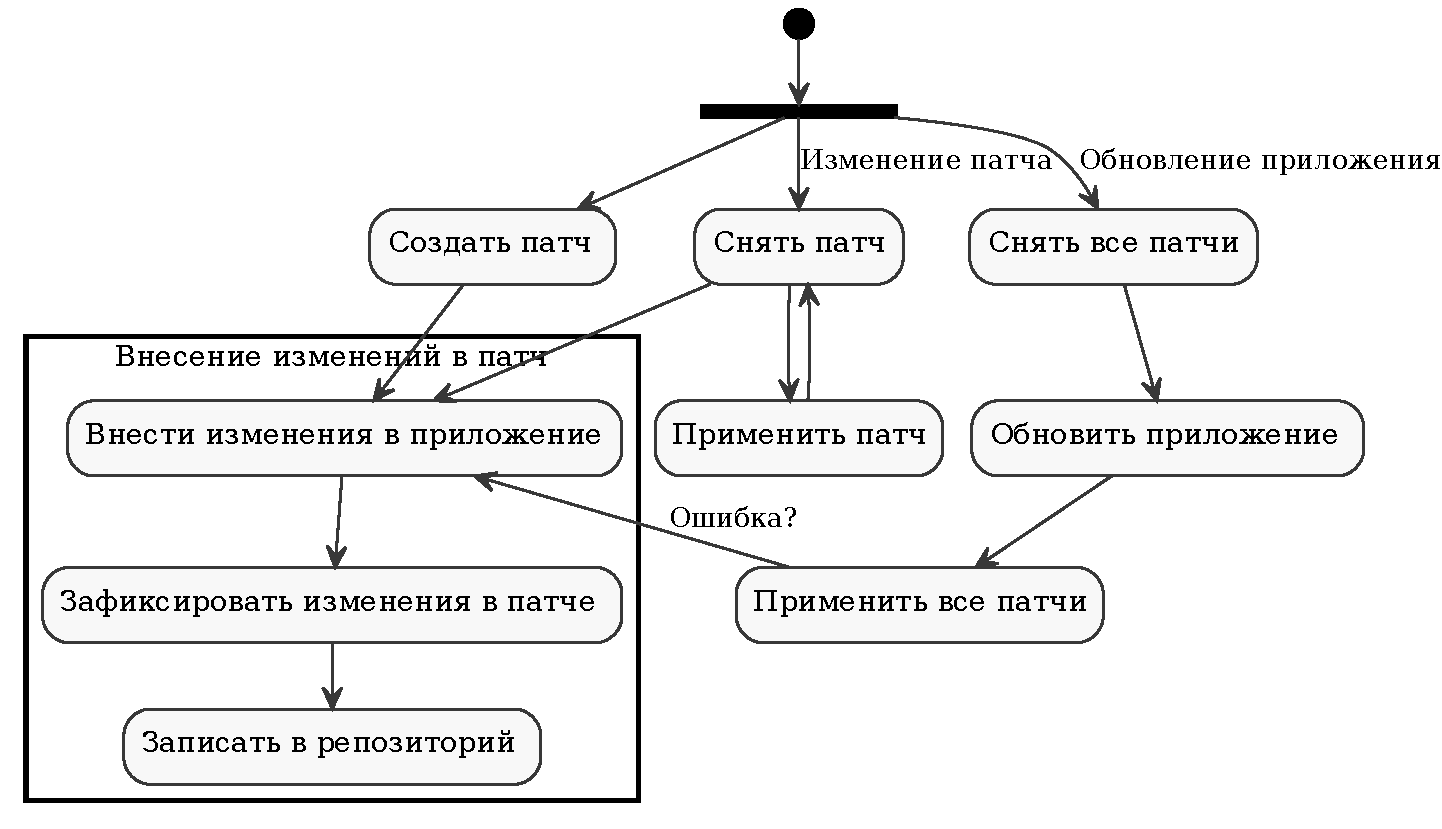
\includegraphics[width=1\textwidth]{mq-workflow.pdf}}
\end{frame}

\begin{comment} 
Следующим шагом была проведена работа по усовершенствованию
процесса поддержки расширений. Для достижение данной цели все расширения были
единообразно оформлены в виде патчей. Патчи это текстовый файл в которым
отражены изменения исходного кода, в виде добавленных и удалённых строк. Патч
применяется к исходным кодам приложения тем самым модифицируя его.

В автоматизация процесса был использован инструмент Mercurial Queues, являющийся
модулем в системе контроля версий Mercurial. Он автоматизирует операции,
связанные с управлением патчами, а также позволяет хранить историю их 
изменений.

На слайде показан процесс, который был создан для поддержки расширений.
Существует три сценария работы: создание и изменение патча и обновление
приложения. Процессы cоздание и изменения патча похожи. В первую очередь
производится создание нового или выбор патча с которым будет осуществляться
работа, затем вносятся изменения в исходные коды приложения. По окончании
изменения записываются в патч и сохраняются в репозитории.

При обновлении приложения все патчи снимаются, приложение обновляется и патчи
применяются заново. Если возникает ошибка при установке патча, то производится
изменение данного патча и запись этих изменений в репозиторий. Шаг повторяется
до тех пор, пока все патчи не будут успешно адаптированы под новую версию
приложения.

С помощью инструмента Mercurial Queues была автоматизирована установка плагинов
и патчей, а также он был успешно внедрён в процесс разработки
расширений, что позволило снизить трудозатраты на поддержку расширений.

\end{comment}


\begin{frame}
\transwipe[direction=90]
\frametitle{Расширение на хостинге Github}
\centerline{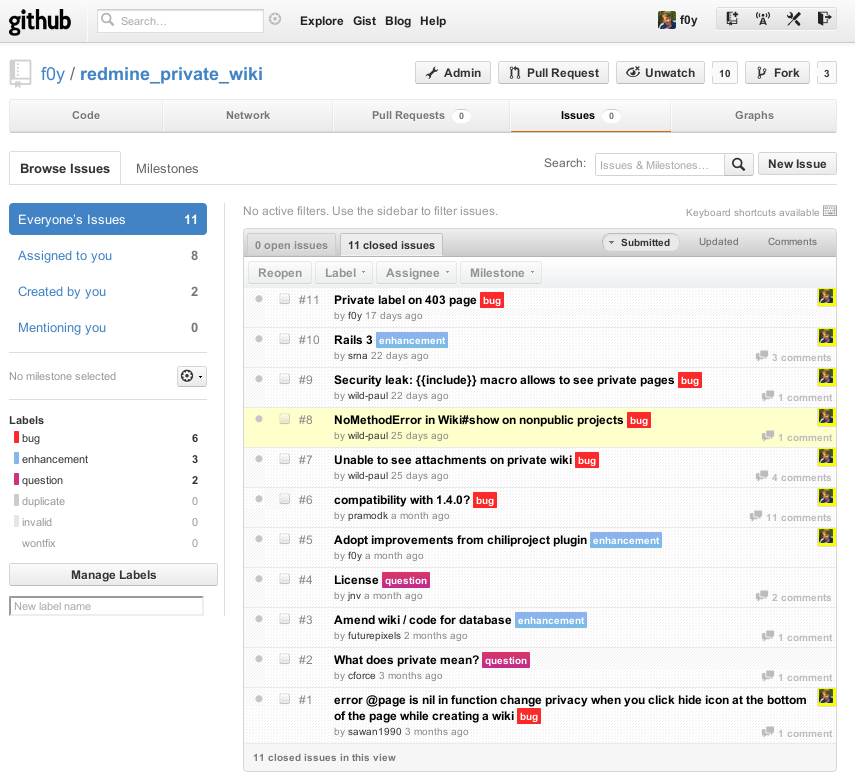
\includegraphics[scale=0.4]{private-wiki-on-github.png}}
\end{frame}

\begin{comment}

На слайде отображена страница с одним из плагинов на хостинге проектов гитхаб.

Исходные коды расширений были размещены в открытом доступе. Один из патчей был
размещен на официальном сайте Redmine и ждёт рассмотрения на принятие в кодовую
базу проекта. Патч, который вносит улучшения в плагин для обзора кода, был
принят автором плагина и текущая версия плагина уже содержит данное улучшение.

Исходные коды 4 разработанных плагинов выложены на хостинг проектов github. Был
произведён анонс одного из плагинов, для того, чтобы привлечь пользователей.
При помощи подобной рекламы было получено было получено 6 отзывов и 3 патча от
8 пользователей. Списое отзывов и патчей отображены на слайде.
Полученные патчи были приняты в кодовую базу плагина, а на основе отзывов
внесены улучшения. Стоит отметить, что один из пользователей портировал плагин
в схожую систему управления проектов и внёс множество улучшений, которые в
последствии были перенесены в оригинальный плагин.

Таким образом плагин доказал свою востребованность, а взаимодействие с
сообществом позволило улучшить его качество.
 
\end{comment}


\begin{frame}
\transwipe[direction=90]
\frametitle{Результаты}
\begin{block}{Достигнутые результаты}
\begin{itemize}
  \item Разработано 4 плагина и 2 патча \\ 
    \textbf{Добавлен и усовершенствован функционал}
    \vspace{8pt}
  
  \item Создан и внедрён процесс, упрощающий поддержку расширений \\
    \textbf{Cнижены трудозатраты на поддержку}
    \vspace{8pt}
  
  \item Расширения размещены в открытом доступе \\
    \textbf{Улучшено качество плагинов}
    \vspace{8pt}
  
  \item Расширения внедрены в лабораторию FRUCT \\
    \textbf{Повышена эффективность и удобство работы над проектами внутри
  лаборатории}
\end{itemize}
\end{block}
\end{frame}

\begin{comment}

--- Перечислить все пункты ---

\end{comment}


\end{document}